\documentclass[sigconf,nonacm]{acmart}

\usepackage{booktabs}
\usepackage{graphicx}
\usepackage{amsmath}
\usepackage{multirow}
\usepackage{xcolor}
\usepackage{balance}
\usepackage{enumitem}

% Remove ACM-specific metadata
\settopmatter{printacmref=false}
\renewcommand\footnotetextcopyrightpermission[1]{}
\pagestyle{plain}

\begin{document}

\title{Predicting Resolution Time for Municipal Service Requests\\
Using Gradient Boosting: A Study of Boston 311 Data}

\author{Yash Chavan}
\affiliation{%
  \institution{Northeastern University}
  \department{M.S. in Artificial Intelligence}
  \city{Boston}
  \state{MA}
  \country{USA}
}

\begin{abstract}
Municipal 311~systems generate millions of geocoded, timestamped
service requests annually, forming a rich spatial-temporal record
of urban service demand and delivery. This paper addresses the
problem of predicting how long a newly created 311~service request
will take to resolve, using only information available at the time
of request creation. A dataset of 1.82~million closed requests
from the City of Boston spanning 2015--2024 is used, with a strict
temporal train/validation/test split that prevents future
information leakage.

A feature engineering pipeline produces 99~features across ten
categories---temporal, categorical, geographic, historical,
workload, backlog, velocity, interaction, SLA~baseline, and
velocity deviation---all respecting a creation-time information
boundary. Geographic features encode the spatial context of each
request, while operational features capture department-level and
neighborhood-level service dynamics with appropriate causal lags.

Twenty-two model configurations across six model families are
systematically evaluated, including statistical baselines, linear
models, Random Forest, and three gradient boosting frameworks
(XGBoost, LightGBM, CatBoost) with robust loss functions, Optuna
hyperparameter optimization, hurdle models, and blended ensembles.
The best model, CatBoost with MAE loss, achieves a mean absolute
error (MAE) of 2.67~days on the held-out 2023--2024 test set,
representing a 33.3\% reduction over the mean baseline
(MAE\,=\,4.00\,d) and a 24.8\% reduction over the best
SARIMA model (MAE\,=\,3.55\,d). Walk-forward validation across
three annual folds confirms temporal stability
(MAE range 2.43--2.66\,d).

SHAP-based feature importance analysis reveals that
target-encoded service queue attributes and category-level
resolution statistics dominate, while purely geographic features
contribute modestly---suggesting that the spatial signal in
311 resolution
time operates primarily through the organizational and categorical
structure of municipal service delivery rather than through raw
location coordinates. On the Boston dataset studied here, per-request
machine learning considerably outperforms aggregate time-series
forecasting, while the analysis also identifies a performance
plateau attributable to irreducible operational variance absent
from the available data.
\end{abstract}

\keywords{311 service requests, resolution time prediction,
gradient boosting, urban computing, spatial-temporal analytics,
municipal service delivery}

\maketitle

%% ================================================================
\section{Introduction}
\label{sec:intro}
%% ================================================================

Municipal 311~systems serve as centralized intake channels for
non-emergency city service requests, handling issues such as
potholes, broken streetlights, graffiti, sanitation complaints,
and noise violations. In the United States alone, major cities
collectively process millions of 311~requests per year, each
generating a geocoded, timestamped record that captures the type
of issue, its location, the responsible department, and the
eventual resolution outcome. This data forms a uniquely granular
spatial-temporal record of how cities deliver services across
their geographic footprint~\cite{zheng2014urban,
wang2017structure311}.

Predicting how long a newly submitted 311~request will take to
resolve has direct practical value. Accurate predictions enable
city agencies to prioritize dispatch, allocate resources to
overburdened departments or neighborhoods, and set realistic
expectations for residents. From a spatial analytics perspective,
resolution time is a measurable proxy for service delivery
efficiency that varies systematically across space, time, and
request category~\cite{wang2017structure311}---making it a natural
target for spatial-temporal prediction methods.

Prior work on 311~analytics has explored request classification
\cite{kim2021classification311}, 311~request composition as a
signature of urban location~\cite{wang2017structure311},
socio-spatial disparities in reporting
behavior~\cite{kontokosta2021bias}, and aggregate volume
prediction~\cite{cheng2022311ml}. The most directly related
system, SWIFT~\cite{raj2021swift}, predicts weekly aggregate
resolution times using sparse Gaussian Conditional Random Fields
(GCRFs) with a two-week historical lookback. That approach
forecasts period-level averages rather than individual request
outcomes, limiting its utility for real-time per-request triage.

This study takes a complementary approach: predicting resolution
time at the \emph{individual request level} using per-request
features available at creation time. The contributions are:

\begin{enumerate}[leftmargin=*,nosep]
\item A 99-feature engineering pipeline covering temporal,
      categorical, geographic, historical, workload, and
      interaction dimensions, all respecting a strict
      creation-time information boundary that prevents
      temporal leakage.
\item A systematic comparison of 22~model configurations
      across six model families---statistical baselines, linear
      models, Random Forest, XGBoost, LightGBM, and
      CatBoost---including robust loss functions, Optuna-tuned
      hyperparameters, hurdle models, and blended ensembles.
\item A methodological bridge between per-request ML and
      aggregate time-series forecasting (ARIMA/SARIMA),
      contextualizing the results relative to SWIFT's
      time-series approach.
\item Empirical characterization of the performance plateau
      imposed by irreducible operational variance, providing
      evidence that further gains require richer data sources
      rather than more complex models.
\item SHAP-based interpretability analysis revealing how spatial,
      temporal, and organizational features contribute to
      prediction accuracy.
\end{enumerate}

The remainder of this paper is organized as follows.
Section~\ref{sec:related} reviews related work on 311~analytics,
urban service prediction, and gradient boosting.
Section~\ref{sec:formulation} formally defines the prediction
task and evaluation protocol. Section~\ref{sec:data} describes
the dataset and preprocessing pipeline. Section~\ref{sec:features}
details the feature engineering approach with emphasis on
spatial-temporal features. Section~\ref{sec:design} presents the
experimental design. Section~\ref{sec:results} reports results
across all model configurations. Section~\ref{sec:discussion}
discusses findings in the context of prior work and deployment
considerations. Section~\ref{sec:limitations} acknowledges
limitations, and Section~\ref{sec:conclusion} concludes with
directions for future work.

%% ================================================================
\section{Related Work}
\label{sec:related}
%% ================================================================

\subsection{311 Service Request Analytics}

The 311~system has become a significant data source for urban
analytics research. Wang et al.~\cite{wang2017structure311}
demonstrate that the composition of 311~request types within a
geographic area acts as a ``signature'' of that location,
encoding meaningful socioeconomic and land-use information across
New York City, Boston, and Chicago. This finding supports the use
of category-level and neighborhood-level features for prediction
tasks on 311~data.

Kim and Hong~\cite{kim2021classification311} apply deep learning
to classify transportation-related 311~requests in Boston
(2016--2018), addressing class imbalance challenges inherent in
citizen-reported data. Cheng et al.~\cite{cheng2022311ml} use
machine learning to analyze 311~request patterns in Miami-Dade
County at the census-tract level, though their focus is on volume
prediction and community characteristics rather than resolution
time.

Kontokosta and Hong~\cite{kontokosta2021bias} examine
socio-spatial disparities in 311~complaint behavior, finding that
low-income and minority neighborhoods systematically under-report
relative to need. This work provides important context for
interpreting any spatial patterns in 311~prediction models, as
the training data reflects reporting behavior rather than
ground-truth service need.

However, none of these studies address the problem of predicting
resolution time at the individual request level---the gap that
motivates the present work.

\subsection{Resolution Time and Service Time Prediction}

SWIFT~\cite{raj2021swift} is the most directly comparable prior
system. It predicts weekly aggregate response times for
non-emergency service requests using sparse GCRFs, comparing
against ARIMA~\cite{box1970arima} and linear regression baselines
at weekly granularity. Table~\ref{tab:litcomp} provides a
detailed comparison between SWIFT and the present study.

In the broader domain of service time prediction, Ruan et
al.~\cite{ruan2022servicetime} address last-mile delivery service
time prediction using spatial meta-learning, tackling challenges
of location heterogeneity and skewed observations that are
analogous to those encountered in 311~resolution time prediction.
Their work demonstrates the value of spatial context for service
duration estimation.

\subsection{Gradient Boosting for Tabular Regression}

Gradient boosting decision trees (GBDTs) represent the dominant
paradigm for supervised learning on tabular data. XGBoost
\cite{chen2016xgboost} introduced sparsity-aware splitting and
regularized objectives. LightGBM~\cite{ke2017lightgbm} improved
training efficiency through gradient-based one-side sampling
(GOSS) and exclusive feature bundling (EFB).
CatBoost~\cite{prokhorenkova2018catboost} introduced ordered
boosting and native categorical feature processing to address
target leakage in categorical encoding---directly relevant to
311~data, which contains high-cardinality categorical attributes
such as request type, department, and neighborhood.

Recent benchmarks confirm that tree-based methods consistently
outperform deep learning on medium-sized tabular data.
Grinsztajn et al.~\cite{grinsztajn2022trees} evaluate
45~datasets and identify key inductive biases---robustness to
uninformative features, preservation of feature orientation, and
capacity for irregular function shapes---that favor tree-based
models on tabular data. Shwartz-Ziv and
Armon~\cite{shwartzziv2022tabular} reach similar conclusions,
finding that XGBoost matches or exceeds deep models on standard
tabular benchmarks. These findings motivate the focus on gradient
boosting methods in this study.

\subsection{Time-Series vs.\ Machine Learning Forecasting}

The M4~Competition~\cite{makridakis2020m4}, which evaluated
61~methods on 100{,}000 time series, found that hybrid approaches
combining statistical and machine learning methods outperformed
pure approaches from either paradigm. Kontopoulou et
al.~\cite{kontopoulou2023arima} review ARIMA versus machine
learning across multiple application domains and find that ML
methods display superior prediction performance in most settings,
though ARIMA remains competitive for short, stationary series.

The ARIMA/SARIMA comparison in this study
(Section~\ref{sec:arima}) serves as a methodological bridge to
SWIFT's time-series approach, while acknowledging the inherent
granularity asymmetry between per-request ML and aggregate
time-series forecasting.

\subsection{Feature Engineering and Interpretability}

Target encoding~\cite{micci2001target} replaces high-cardinality
categorical variables with smoothed conditional means of the
target, providing a principled approach to encoding variables like
request type and department that may have hundreds of unique
values. Careful use of training-set-only statistics and smoothing
parameters prevents target leakage.

SHAP (SHapley Additive exPlanations)~\cite{lundberg2017shap}
provides a game-theoretically grounded framework for feature
attribution. The TreeSHAP algorithm~\cite{lundberg2020treeshap}
enables exact, polynomial-time computation of SHAP values for
tree-based models, supporting both local explanation of individual
predictions and global understanding of feature importance
patterns.

\subsection{Comparative Positioning}

Table~\ref{tab:litcomp} summarizes the key differences between
this study and the most directly comparable prior work. The
primary distinction from SWIFT is the shift from weekly aggregate
forecasting to individual-request prediction with a substantially
richer feature set.

\begin{table*}[t]
\caption{Comparison with the most directly related prior work on
311 resolution time prediction.}
\label{tab:litcomp}
\centering
\small
\begin{tabular}{p{3.2cm}p{6.2cm}p{6.2cm}}
\toprule
\textbf{Dimension} & \textbf{SWIFT}~\cite{raj2021swift} &
  \textbf{This Study} \\
\midrule
City / scope & Multiple U.S.\ cities &
  Boston, MA (single city, 10-year span) \\
Data volume & Varies by city; $\sim$3.5 years per city &
  1,823,856 closed requests over 2015--2024 \\
Prediction target & Weekly aggregate resolution time &
  Individual request resolution time (days) \\
Prediction horizon & One week ahead, two-week lookback &
  At request creation time (zero delay) \\
Core method & Sparse Gaussian Conditional Random Fields &
  Gradient boosting (CatBoost, LightGBM, XGBoost) \\
Feature approach & Two-week historical time-series &
  99 per-request features (temporal, categorical,
  geographic, historical, operational) \\
Spatial features & Temporal aggregates only &
  Lat/lon, distance from city center, neighborhood-level
  backlog, department--neighborhood interactions \\
Baselines compared & ARIMA, linear regression &
  Mean/median, linear models, Random Forest, ARIMA/SARIMA,
  22 total configurations \\
Evaluation & MAE on weekly aggregates &
  MAE on individual requests (2023--2024 test set) \\
Interpretability & Not reported &
  SHAP feature importance (TreeSHAP) \\
Temporal validation & Not reported &
  Walk-forward across 3 annual folds \\
\bottomrule
\end{tabular}
\end{table*}

Direct numeric comparison between the two approaches is not
possible due to differences in city, time period, prediction
granularity, and evaluation protocol. The ARIMA/SARIMA comparison
in Section~\ref{sec:arima} provides an indirect methodological
bridge, demonstrating the advantage of per-request ML over the
aggregate time-series paradigm that SWIFT extends.

%% ================================================================
\section{Problem Formulation}
\label{sec:formulation}
%% ================================================================

\subsection{Task Definition}

Given a newly created 311~service request~$r$ with observable
attributes available at creation time, the task is to predict
$y(r)$, the resolution time in days, defined as:
\begin{equation}
y(r) = \frac{\texttt{CLOSED\_DT}(r) - \texttt{OPEN\_DT}(r)}{86400}
\end{equation}
where timestamps are in seconds. The prediction must use only
features~$\mathbf{x}(r)$ derivable from information available at
or before the creation time~$\texttt{OPEN\_DT}(r)$.

\subsection{Information Boundary}

A strict \emph{creation-time information boundary} governs all
features: no feature for request~$r$ may depend on the closed
date, resolution time, or any post-creation event of~$r$~itself.
Features derived from historical patterns (e.g., mean resolution
time for a request type) use only data from the training period.
Operational features such as department backlog use a one-day lag
on close dates to prevent same-day information leakage.

\subsection{Evaluation Metrics}

The primary evaluation metric is mean absolute error (MAE) in the
original day scale. Secondary metrics include $R^2$
(coefficient of determination) and RMSE. Following Hyndman and
Koehler~\cite{hyndman2006mase}, MASE is also computed, though
its interpretation requires care because the denominator used is
the test-set mean absolute deviation (MAD) rather than the
training-set mean baseline MAE.

All metrics are computed after back-transforming predictions from
the $\log(1+x)$~scale used for training to the original day
scale. Percentage improvement is reported relative to the mean
baseline~(MAE\,=\,4.00\,d).

%% ================================================================
\section{Data}
\label{sec:data}
%% ================================================================

\subsection{Source and Scope}

The dataset comprises all 311~service requests recorded by the
City of Boston from January~2015 through December~2024, obtained
from the Boston Open Data Portal (\texttt{data.boston.gov}). The
raw dataset contains 2,550,536~records across 10~annual files.
Each record includes a geocoded location (latitude, longitude),
timestamps for creation and closure, the request type and
category (REASON), the responsible department, and the
neighborhood.

\subsection{Filtering Pipeline}

Table~\ref{tab:filtering} summarizes the filtering stages. Cases
are restricted to closed requests with valid dates, non-negative
resolution times, a 90-day cap to exclude extreme outliers, and
exclusion of administrative closures (cases closed without
substantive work, e.g., duplicates, automatic closures). The
90-day cap removes 5.5\% of otherwise-valid records and reduces
the influence of extreme outliers on both training and evaluation.
The administrative closure filter removes an additional 17.7\% of
records that do not represent genuine service delivery.

\begin{table}[t]
\caption{Data filtering pipeline.}
\label{tab:filtering}
\centering
\small
\begin{tabular}{lrr}
\toprule
\textbf{Stage} & \textbf{Records} & \textbf{Dropped} \\
\midrule
Raw data                & 2,550,536 & ---     \\
Closed cases only       & 2,348,040 & 202,496 \\
Valid dates             & 2,348,038 & 2       \\
Non-negative resolution & 2,347,246 & 792     \\
90-day cap              & 2,217,370 & 129,876 \\
Remove admin.\ closures & 1,823,856 & 393,514 \\
\bottomrule
\end{tabular}
\end{table}

\subsection{Target Variable}

The prediction target is resolution time in days. The
distribution is heavily right-skewed (Figure~\ref{fig:target}):
mean\,=\,4.50\,d, median\,=\,0.47\,d,
standard deviation\,=\,11.59\,d, skewness\,=\,4.23.
Approximately 64\% of requests resolve within one day, while the
remaining 36\% span up to the 90-day cap. A
$\log(1+x)$~transformation is applied during training to
compress the right tail; all reported metrics use
back-transformed predictions in the original day scale.

\begin{figure}[t]
\centering
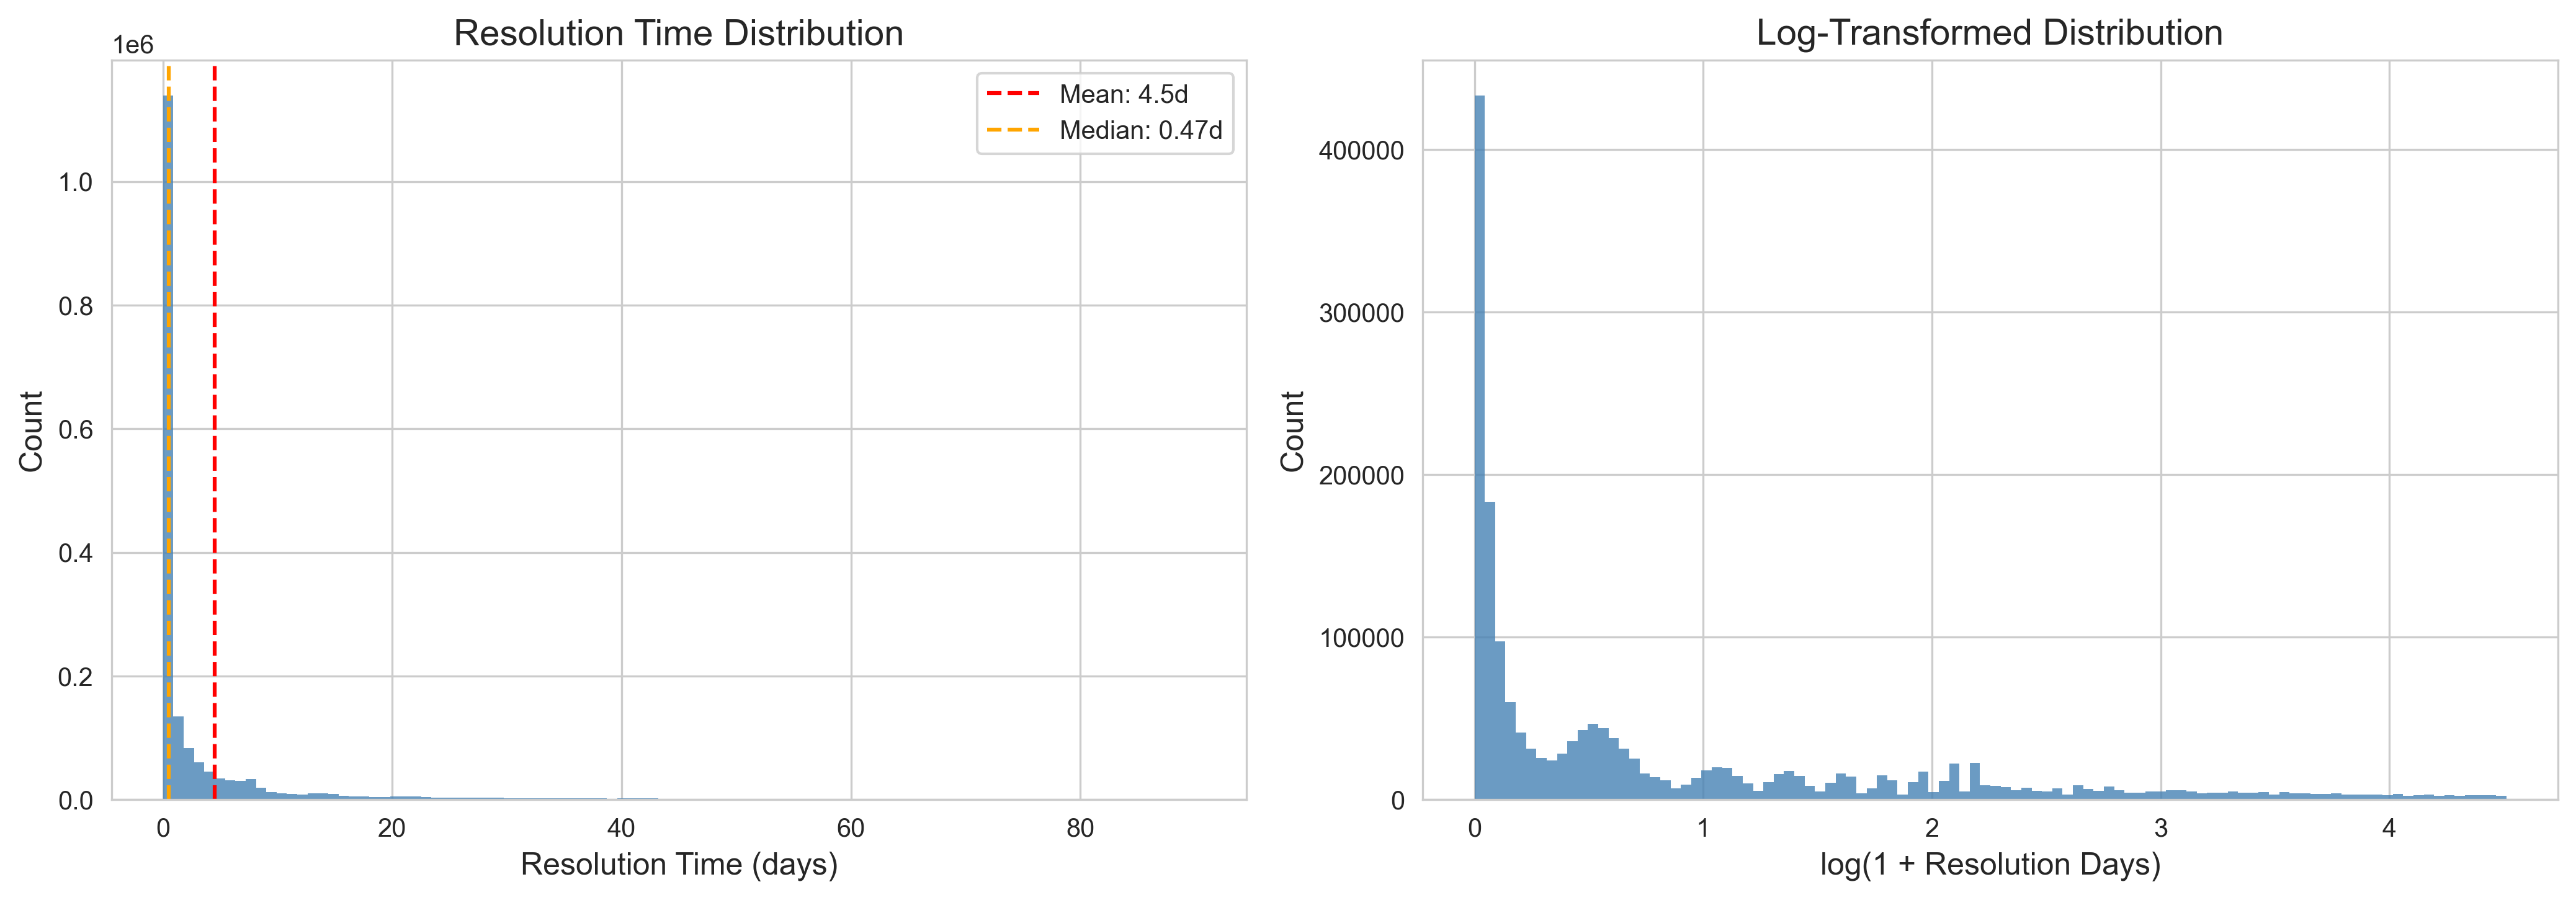
\includegraphics[width=\columnwidth]{figures/eda_resolution_distribution.png}
\caption{Distribution of resolution time (days) for the
1.82\,M filtered requests. The distribution is heavily
right-skewed with 64\% of cases resolving within one day.}
\label{fig:target}
\end{figure}

The extreme skewness of the target has two important consequences
for modeling. First, MAE is dominated by the majority of
short-resolution cases, making it difficult for models to
simultaneously minimize error on both short and long cases.
Second, $R^2$ values are structurally low because the total
variance is inflated by the heavy right tail, even when
predictions are reasonably accurate in absolute terms.

\subsection{Temporal Split}

A strict temporal split prevents future information from leaking
into training (Table~\ref{tab:split}). The training set covers
2015--2021, the validation set covers 2022, and the test set
covers 2023--2024.

\begin{table}[t]
\caption{Temporal data split.}
\label{tab:split}
\centering
\small
\begin{tabular}{llrr}
\toprule
\textbf{Split} & \textbf{Years} & \textbf{Records} & \textbf{\%} \\
\midrule
Train      & 2015--2021 & 1,190,355 & 65.3 \\
Validation & 2022       &   224,371 & 12.3 \\
Test       & 2023--2024 &   409,130 & 22.4 \\
\bottomrule
\end{tabular}
\end{table}

\subsection{Nested Selection Protocol}

Within the training block, year~2021 is held out as a
\emph{tune fold} for all model selection decisions: loss function
sweeps, Optuna hyperparameter tuning, ensemble weight
optimization, and hurdle threshold selection. The train-proper
subset (2015--2020) is used to fit candidate models, and the tune
fold (2021) is used to compare them. The validation set (2022) is
reserved exclusively for early-stopping callbacks during gradient
boosting training---it is never used for model selection. This
nested design prevents the validation set from implicitly
participating in selection, a subtle form of leakage that can
inflate reported performance.

After selection, final models are retrained on the full training
block (2015--2021) with the validation set (2022) providing
early stopping. The test set (2023--2024) is evaluated only once
per model.

\subsection{Spatial Distribution}

Boston's 311~requests are distributed across approximately 25
neighborhoods with substantial variation in request volume and
type composition. High-volume neighborhoods (Dorchester,
Roxbury, South Boston) generate disproportionately more requests,
while request type distributions vary geographically---e.g.,
snow-related requests concentrate in residential neighborhoods,
while commercial-area complaints cluster in downtown districts.
This spatial heterogeneity motivates the inclusion of
neighborhood-level features in the prediction pipeline.

%% ================================================================
\section{Feature Engineering}
\label{sec:features}
%% ================================================================

All 99~features respect the creation-time information boundary
defined in Section~\ref{sec:formulation}. No feature uses the
closed date, resolution time, or any post-creation event of the
request being predicted. Table~\ref{tab:features} provides an
overview.

\begin{table}[t]
\caption{Feature categories (99 total).}
\label{tab:features}
\centering
\small
\begin{tabular}{lrl}
\toprule
\textbf{Category} & \textbf{N} & \textbf{Examples} \\
\midrule
Temporal           & 27 & hour, day\_of\_week, cyclical  \\
                   &    & sin/cos, holiday, season       \\
Categorical (enc.) & 26 & Target + frequency encoding    \\
                   &    & for 13 columns                 \\
Geographic         &  5 & lat, lon, dist.\ from center,  \\
                   &    & zipcode, has\_coordinates       \\
Historical agg.    & 15 & mean/median/std by TYPE,       \\
                   &    & REASON, Dept (train only)      \\
Workload proxy     &  2 & prev-day/week request counts   \\
District backlog   &  2 & open cases per neighborhood    \\
                   &    & and department (1-day lag)      \\
Dept.\ velocity    &  6 & rolling 7/14/30-day avg        \\
                   &    & resolution by TYPE, Dept       \\
Interaction        &  8 & type$\times$dept, velocity     \\
                   &    & $\times$backlog, backlog ratio \\
SLA baseline       &  6 & P25/P75/IQR per TYPE, REASON   \\
Velocity deviation &  2 & current vs.\ historical speed  \\
\bottomrule
\end{tabular}
\end{table}

\subsection{Temporal Features}

Twenty-seven features capture the temporal context of request
creation. Basic extractions include hour of day, day of week,
month, quarter, year, and day of year. Cyclical sine/cosine
transformations are applied to hour, day of week, month, and
day of year to preserve periodicity at boundaries. Binary indicators flag weekends, holidays (U.S.\
federal), business hours (9\,AM--5\,PM weekdays), and seasonal
categories (spring, summer, fall, winter). Time-of-day buckets
(morning, afternoon, evening, night) provide coarser temporal
groupings.

\subsection{Categorical Encoding}

Thirteen categorical columns (TYPE, REASON, Department,
neighborhood, Source, ward, voting precinct, and others) are
encoded using two complementary strategies.
\emph{Target encoding}~\cite{micci2001target} replaces each
category level with the smoothed mean of the log-transformed
target in the training set, using a smoothing parameter of~10 to
regularize low-count categories. \emph{Frequency encoding}
replaces each level with its relative frequency in the training
set. Both encoders are fitted exclusively on training data and
applied to validation and test sets; unseen categories fall back
to the global mean (target encoding) or zero (frequency
encoding). This yields 26~encoded features (2 per column for the
13~columns).

\subsection{Geographic and Spatial Features}

Five features capture the spatial context of each request:
raw latitude and longitude, a binary indicator for whether
coordinates are available (\texttt{has\_coordinates}), the
zipcode, and Euclidean distance from Boston's approximate city
center (42.36$^\circ$N, 71.06$^\circ$W). The Euclidean
approximation on geographic coordinates introduces modest
distortion at Boston's latitude ($\sim$26\% longitude
compression), but this does not affect tree-based model
performance, which depends on threshold ordering rather than
absolute distances.

The spatial signal in 311~resolution time is hypothesized to
operate indirectly: location determines which department handles
a request, what infrastructure surrounds it, and what historical
service patterns exist in that area. Rather than encoding spatial
proximity directly, the pipeline captures these indirect effects
through neighborhood-level backlog, department velocity, and
interaction features.

\subsection{Historical and Operational Features}

Fifteen \emph{historical aggregate} features encode the mean,
median, and standard deviation of resolution time for each
request TYPE, REASON, and Department, computed from training data
only. These provide strong priors: requests of a type that
historically resolves quickly are likely to resolve quickly again.

Two \emph{workload proxy} features capture the volume of requests
submitted in the previous day and previous week, using a one-day
lag to ensure causal availability. Two \emph{district backlog}
features count the number of currently open cases per
neighborhood and per department, with a one-day lag on close dates
(on day~$D$, only closures through day~$D{-}1$ are subtracted).
This lag ensures that backlog features reflect information that
would genuinely be available in a real-time deployment scenario.

Six \emph{department velocity} features capture rolling 7-, 14-,
and 30-day average resolution times per TYPE and per Department.
These dynamic features track whether a department is currently
resolving cases faster or slower than its historical average,
providing a real-time operational signal.

\subsection{Interaction and Derived Features}

Eight interaction features capture nonlinear relationships:
cross-encodings of type with department and neighborhood,
velocity--backlog products, and backlog ratios. Six SLA~baseline features encode the
25th~percentile, 75th~percentile, and interquartile range of
historical resolution time per TYPE and REASON, providing a
distributional prior beyond the mean. Two velocity deviation
features measure the ratio and difference between current
department velocity and historical averages.

\subsection{Monotonic Constraints}

For models that support them (LightGBM), monotonic constraints
are applied to features with clear directional relationships:
historical mean resolution time is constrained to have a positive
relationship with predicted resolution time, and business-hours
indicators are constrained to have a negative relationship
(requests submitted during business hours tend to resolve faster).
These constraints encode domain knowledge without restricting the
model's ability to capture nonlinear relationships within the
monotonic direction.

%% ================================================================
\section{Experimental Design}
\label{sec:design}
%% ================================================================

\subsection{Model Progression}

Models are evaluated in a staged progression from simple to
complex, establishing clear baselines before introducing
sophistication:

\begin{enumerate}[leftmargin=*,nosep]
\item \textbf{Statistical baselines:} Global mean and median
      predictors (no features used).
\item \textbf{Linear models:} Linear Regression, Ridge,
      Lasso, and Decision Tree (max depth~10).
\item \textbf{Gradient boosting (default hyperparameters):}
      Random Forest~\cite{breiman2001random},
      XGBoost~\cite{chen2016xgboost},
      CatBoost~\cite{prokhorenkova2018catboost}.
\item \textbf{Advanced LightGBM:} Robust loss functions
      (Huber $\delta$\,=\,0.5, Fair $c$\,=\,1, Tweedie
      $p$\,=\,1.5, quantile $\alpha$\,=\,0.5), Optuna-tuned
      hyperparameters, hurdle models, and SLSQP-optimized
      blended ensembles.
\item \textbf{Improvement experiments:} CatBoost with MAE loss
      (GPU), XGBoost with absolute error (CUDA), recency-weighted
      training, and deeper Optuna tuning (50 trials).
\end{enumerate}

\subsection{Loss Function Selection}

The default L2~(MSE) loss penalizes large errors
disproportionately, which can lead to overcompensation on the
heavy-tailed 311~target. Robust alternatives are evaluated:
\textbf{Huber loss} transitions from L2 to L1 beyond a threshold
$\delta$, reducing sensitivity to outliers.
\textbf{Fair loss} provides a smooth approximation to L1.
\textbf{Tweedie loss} models the target as a Tweedie distribution,
natively handling the point mass at zero.
\textbf{Quantile loss} ($\alpha$\,=\,0.5) targets the conditional
median rather than the mean.

Loss function candidates are swept using the nested selection
protocol: models are trained on the train-proper subset
(2015--2020) and evaluated on the tune fold (2021), with the best
configuration retrained on the full training set (2015--2021).

\subsection{Hyperparameter Optimization}

Optuna~\cite{akiba2019optuna} is used with a TPE (Tree-structured
Parzen Estimator) sampler and 30~trials on a 300K-row subsample
with 3-fold \texttt{TimeSeriesSplit} cross-validation. The search
space covers learning rate, number of leaves, minimum child
samples, L1/L2 regularization, feature fraction, bagging fraction,
and maximum depth. The objective minimizes MAE in the original day
scale after $\exp(x)-1$ back-transformation, ensuring that
hyperparameters are optimized for the metric of practical interest
rather than the log-scale training loss.

\subsection{Hurdle Model}

A two-stage hurdle model addresses the bimodal nature of the
target distribution. Stage~1 is a LightGBM binary classifier
separating short-resolution from long-resolution cases at a
threshold selected on the tune fold from
$\{0.5, 1, 3, 7\}$~days. Stage~2 applies separate regressors
for each group. Both \emph{soft gating} (probability-weighted
blend of both regressors) and \emph{hard gating} (deterministic
classifier decision) variants are evaluated.

\subsection{Ensemble Construction}

A weighted blend of five LightGBM variants (quantile, L2 with
monotonic constraints, Huber, Fair, and Optuna-tuned) is
constructed using SLSQP (Sequential Least Squares Programming)
optimization on the tune fold, subject to the constraint that
weights sum to~1 and each weight is non-negative. A
meta-ensemble combining the blend with the hurdle model is also
evaluated.

\subsection{Walk-Forward Validation}

Walk-forward validation tests temporal stability by
sequentially training on all data up to year~$T{-}1$ and testing
on year~$T$, for $T \in \{2022, 2023, 2024\}$. Each fold uses
LightGBM with Huber loss and the same hyperparameters, without
early stopping, to provide a consistent evaluation across folds.

\subsection{ARIMA/SARIMA Comparison Methodology}
\label{sec:arima_method}

To contextualize results against the time-series paradigm used by
SWIFT~\cite{raj2021swift}, ARIMA(2,1,2) and
SARIMA(1,1,1)(1,1,1,52) models are fitted on weekly aggregate
resolution times from the training period. Per-request test
predictions are generated by assigning each request the forecast
for its corresponding calendar week. This methodology allows
MAE comparison on the same test set, though it introduces an
inherent granularity asymmetry: ML models predict individual
outcomes using 99~per-request features, while ARIMA/SARIMA models
assign a single weekly average to all requests in the same week.

%% ================================================================
\section{Results}
\label{sec:results}
%% ================================================================

\subsection{Model Comparison}

Table~\ref{tab:results} presents test-set results for all model
stages. Improvement percentages are relative to the mean baseline
(MAE\,=\,4.00\,d).

\begin{table}[t]
\caption{Test-set results (2023--2024). Improvement is relative
to the mean baseline MAE of 4.00\,d.}
\label{tab:results}
\centering
\small
\begin{tabular}{lccr}
\toprule
\textbf{Model} & \textbf{MAE (d)} & \textbf{$R^2$} &
  \textbf{Impr.} \\
\midrule
Mean baseline         & 4.00 & $-$0.04 &  0.0\% \\
Median baseline       & 3.58 & $-$0.08 & 10.6\% \\
\midrule
Linear Regression     & 2.99 &   0.20  & 25.2\% \\
Ridge                 & 2.99 &   0.20  & 25.2\% \\
Lasso                 & 2.99 &   0.21  & 25.4\% \\
Decision Tree         & 2.93 &   0.25  & 26.7\% \\
\midrule
Random Forest         & 2.83 &   0.29  & 29.3\% \\
XGBoost               & 2.78 &   0.30  & 30.6\% \\
CatBoost (default)    & 2.76 &   0.31  & 31.1\% \\
\midrule
LGB Tuned (Fair)      & 2.70 &   0.33  & 32.6\% \\
LGB Huber             & 2.70 &   0.33  & 32.4\% \\
LGB Quantile          & 2.74 &   0.32  & 31.6\% \\
LGB Fair              & 2.75 &   0.31  & 31.3\% \\
Blended ensemble      & 2.75 &   0.31  & 31.3\% \\
Hurdle (soft, 0.5d)   & 2.75 &   0.29  & 31.2\% \\
LGB L2 + monotonic    & 2.76 &   0.31  & 30.9\% \\
Hurdle (hard, 0.5d)   & 2.81 &   0.35  & 29.7\% \\
LGB Tweedie           & 3.11 &   0.37  & 22.4\% \\
\midrule
\textbf{CatBoost MAE} & \textbf{2.67} & \textbf{0.34} &
  \textbf{33.3\%} \\
XGBoost abs.\ error   & 2.70 &   0.32  & 32.7\% \\
Recency weighting     & 2.71 &   ---   & ---   \\
Deeper Optuna (50)    & 2.73 &   ---   & ---   \\
\bottomrule
\end{tabular}
\end{table}

Several observations emerge from the progression:

\textbf{Diminishing returns.} The largest gains come from the
shift from statistical baselines to linear models (+25\% MAE
reduction) and from linear models to gradient boosting (+5\%
additional). Advanced loss functions and tuning contribute only
an incremental further reduction, consistent with a
data-driven performance plateau.

\textbf{Ensemble collapse.} The SLSQP-optimized blended ensemble
collapsed to 100\% weight on the Fair-loss LightGBM variant,
with all other weights effectively zero. The meta-ensemble
similarly assigned 0\% weight to the hurdle component. This
indicates that the base models produce highly correlated
predictions---unsurprising given that they share the same 99
features and differ only in loss function. True ensemble diversity
would require models with different feature subsets or
fundamentally different architectures.

\textbf{Tweedie underperformance.} Despite its theoretical
suitability for zero-inflated positive targets, LGB~Tweedie
achieves the worst MAE among advanced models (3.11\,d). The
Tweedie distribution's implicit variance--mean relationship does
not match the empirical structure of 311~resolution times, where
variance is not monotonically related to mean duration.

\textbf{CatBoost advantage.} CatBoost with MAE loss achieves the
overall best result (MAE\,=\,2.67\,d, 33.3\% improvement),
outperforming the tuned LightGBM by 0.03\,d. CatBoost's
ordered boosting~\cite{prokhorenkova2018catboost} may provide a
slight advantage by reducing overfitting on this large,
categorically-rich dataset.

\subsection{ARIMA/SARIMA Comparison}
\label{sec:arima}

The comparison of per-request ML against ARIMA/SARIMA baselines
is shown in Table~\ref{tab:arima} and Figure~\ref{fig:arima}.

\begin{table}[t]
\caption{Per-request ML vs.\ ARIMA/SARIMA on the 2023--2024 test
set.}
\label{tab:arima}
\centering
\small
\begin{tabular}{lcc}
\toprule
\textbf{Model} & \textbf{MAE (d)} & \textbf{RMSE (d)} \\
\midrule
\textbf{CatBoost MAE (best ML)} & \textbf{2.67} &
  \textbf{8.67} \\
LGB Tuned (Fair)                & 2.70 &  8.73 \\
SARIMA(1,1,1)(1,1,1,52)        & 3.55 & 11.15 \\
ARIMA(2,1,2) weekly            & 3.55 & 11.14 \\
\bottomrule
\end{tabular}
\end{table}

\begin{figure}[t]
\centering
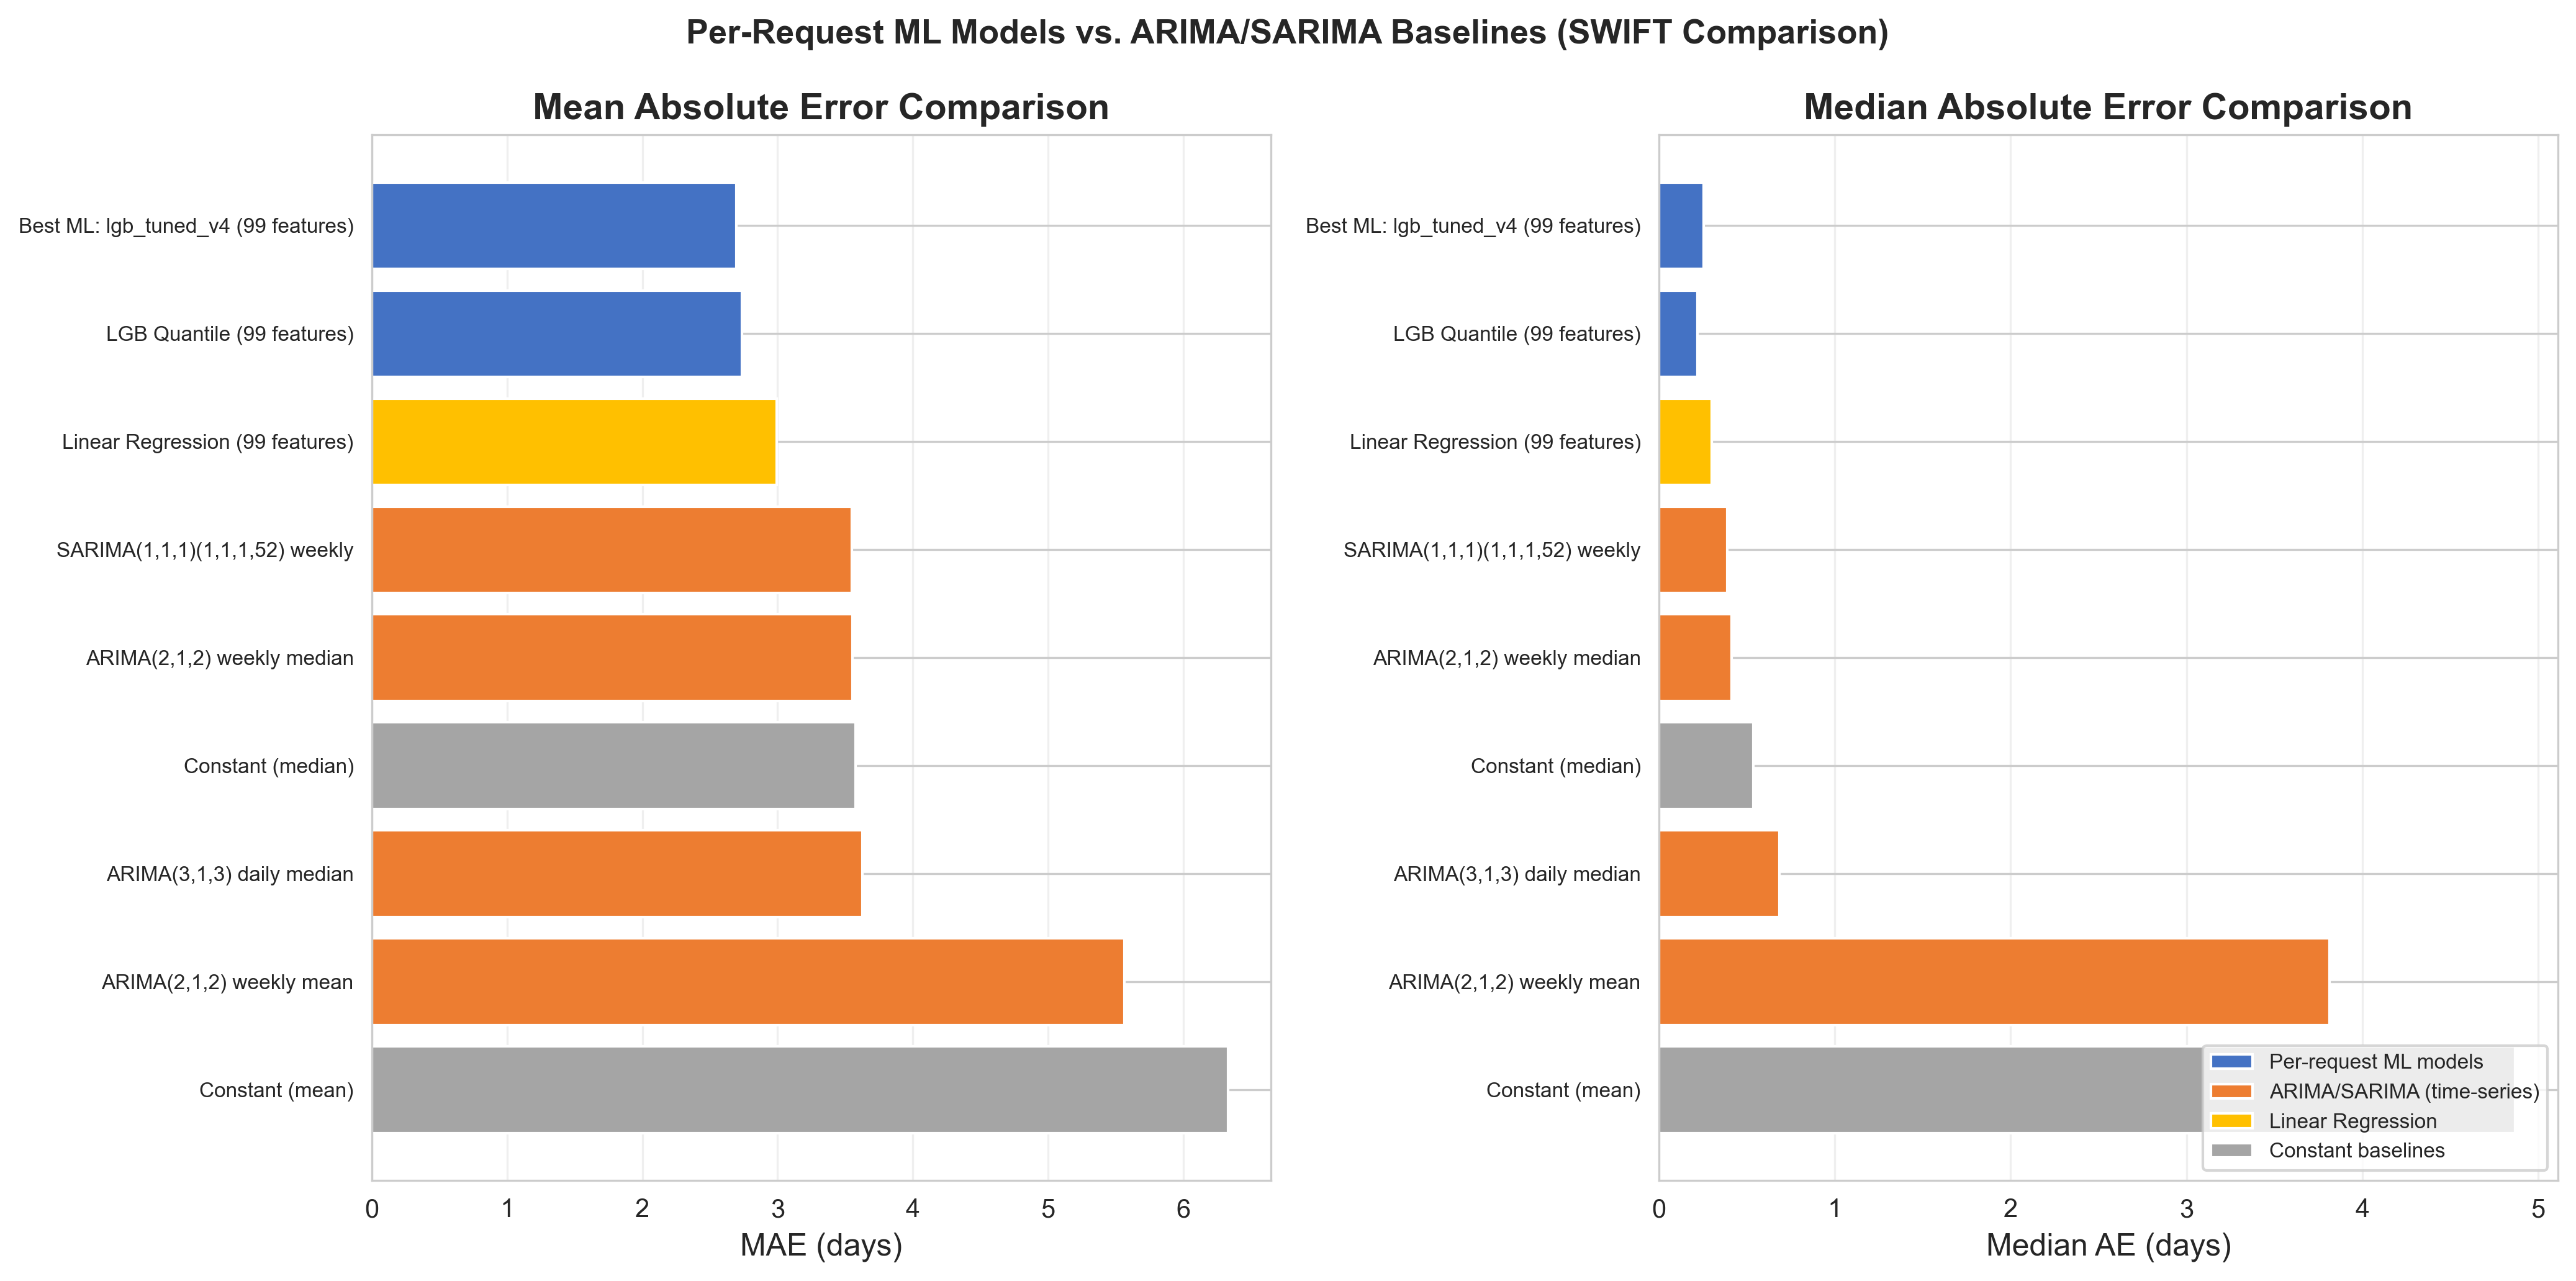
\includegraphics[width=\columnwidth]{figures/arima_comparison.png}
\caption{Per-request ML vs.\ ARIMA/SARIMA baselines on the
2023--2024 test set (left: MAE; right: Median~AE). The ML
model shown is tuned LightGBM.}
\label{fig:arima}
\end{figure}

The best ML model achieves 24.8\% lower MAE than the best SARIMA
model. This comparison has an inherent granularity asymmetry: ML
models predict individual request outcomes using 99~per-request
features, while ARIMA/SARIMA models forecast weekly period
averages and assign the same prediction to all requests in a
given week. The comparison demonstrates that individual-level
prediction with rich features is substantially more informative
than aggregate forecasting, but the 24.8\% figure should be
interpreted with this structural advantage in mind.

Notably, ARIMA and SARIMA produce nearly identical performance
(MAE difference $<$\,0.01\,d), suggesting that the seasonal
component adds negligible value at the weekly aggregation level
for this dataset.

\subsection{Walk-Forward Validation}

Walk-forward validation confirms temporal stability across three
annual test folds (Table~\ref{tab:walkforward},
Figure~\ref{fig:walkforward}).

\begin{table}[t]
\caption{Walk-forward validation results (LightGBM Huber).}
\label{tab:walkforward}
\centering
\small
\begin{tabular}{lccr}
\toprule
\textbf{Test Year} & \textbf{MAE (d)} & \textbf{$R^2$} &
  \textbf{Train Size} \\
\midrule
2022 & 2.43 & 0.31 & 1,190,355 \\
2023 & 2.65 & 0.36 & 1,414,726 \\
2024 & 2.66 & 0.33 & 1,617,961 \\
\bottomrule
\end{tabular}
\end{table}

\begin{figure}[t]
\centering
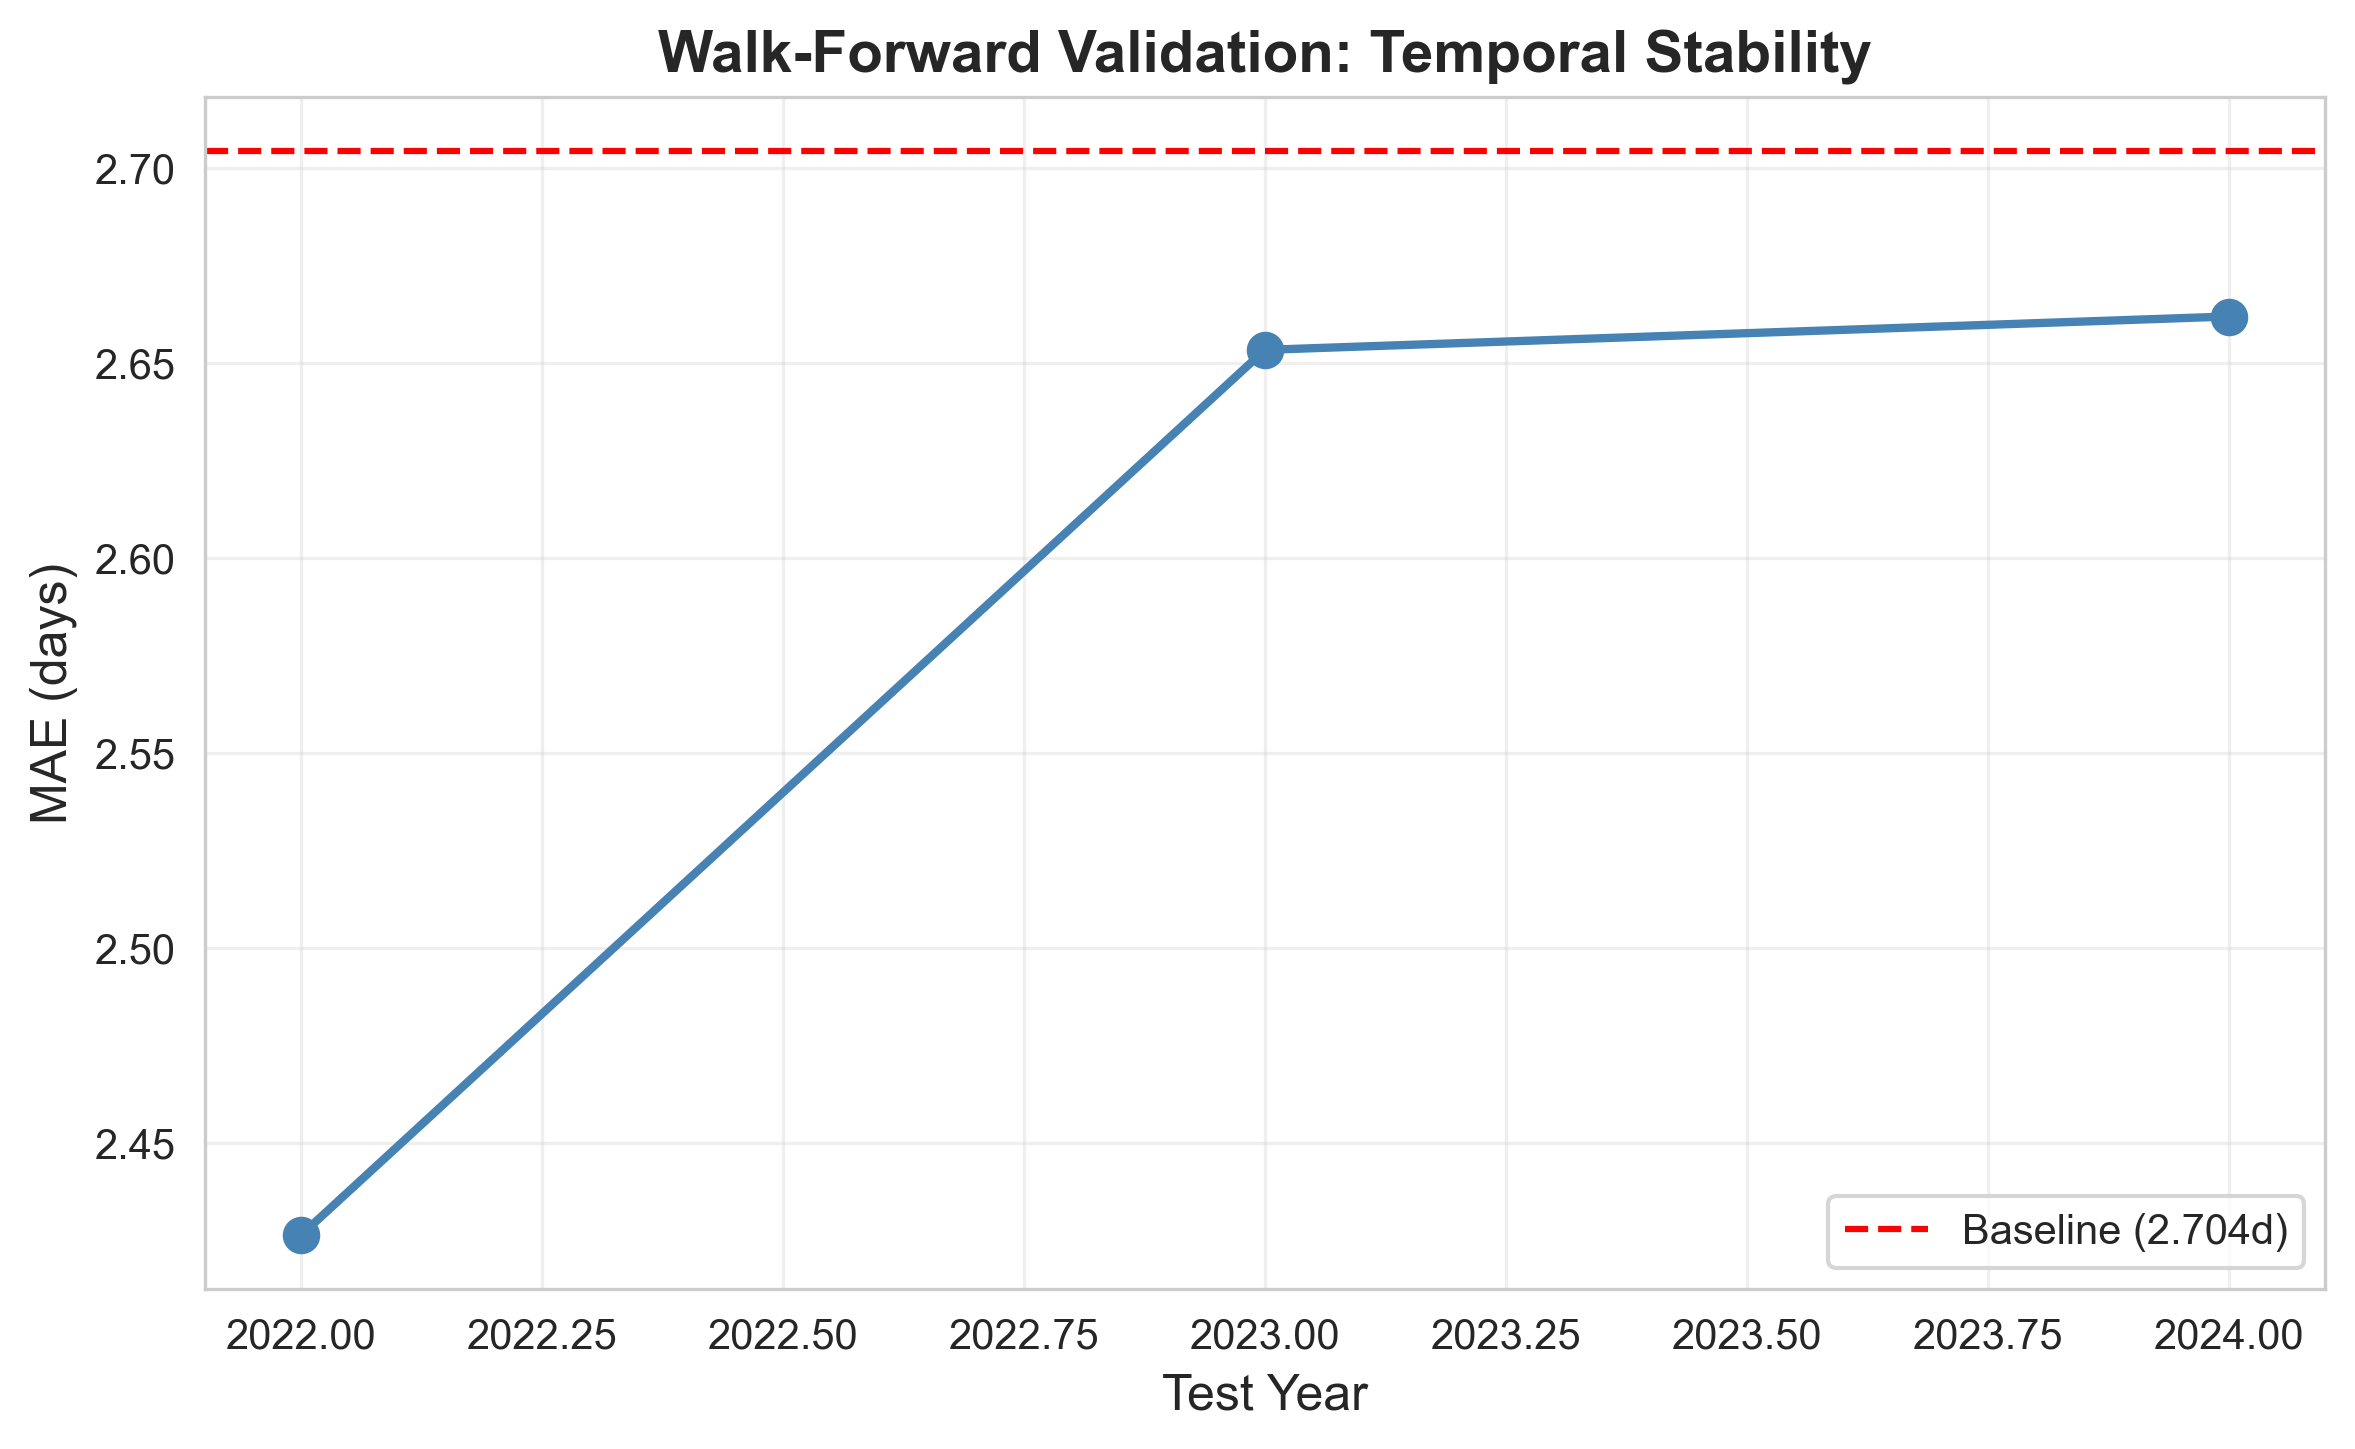
\includegraphics[width=\columnwidth]{figures/walkforward_stability.png}
\caption{Walk-forward MAE across three annual test folds,
demonstrating temporal stability.}
\label{fig:walkforward}
\end{figure}

MAE remains within a narrow range (2.43--2.66\,d) across all
three folds, indicating that model performance does not degrade
as the prediction horizon extends further from the training
period. The lower MAE for 2022 likely reflects distributional
similarity to the 2015--2021 training period rather than a
systematic improvement.

\subsection{Feature Importance}

SHAP analysis~\cite{lundberg2017shap, lundberg2020treeshap}
(Figure~\ref{fig:shap}) reveals the feature importance hierarchy
for the tuned LightGBM model.

\begin{figure}[t]
\centering
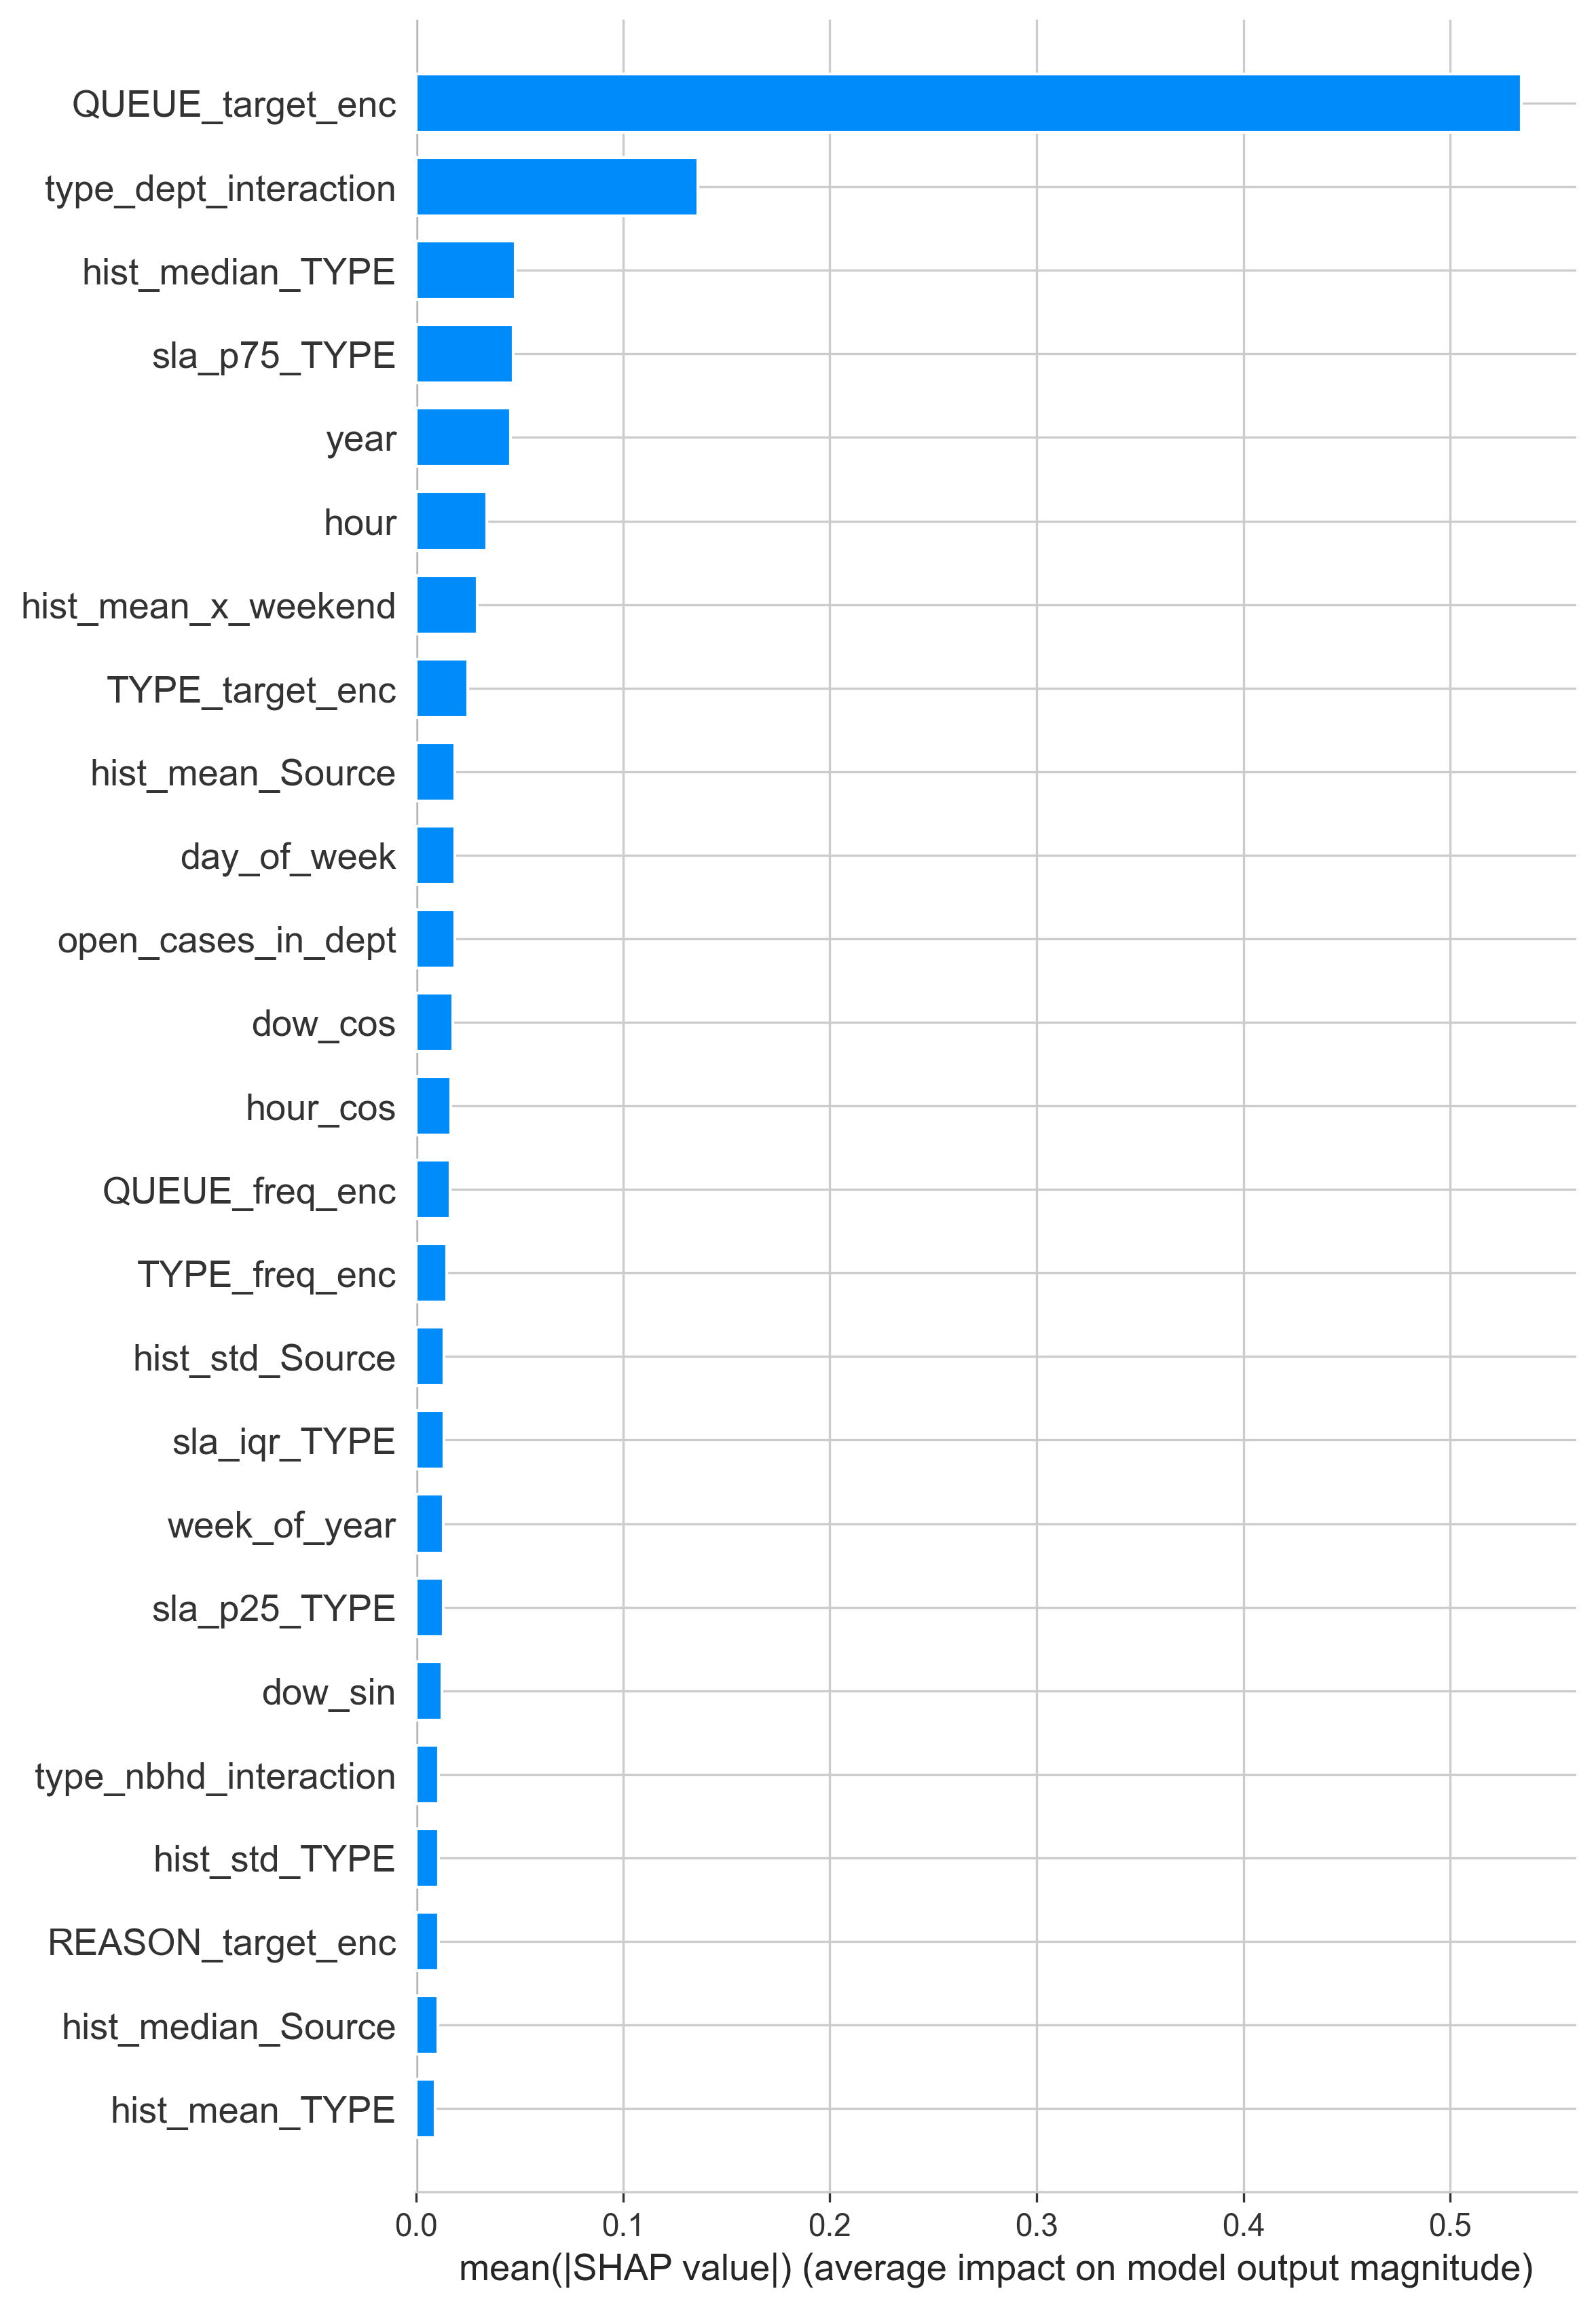
\includegraphics[width=\columnwidth]{figures/shap_importance_v4.png}
\caption{SHAP feature importance (top~25 features, tuned
LightGBM on the test set).}
\label{fig:shap}
\end{figure}

The target-encoded service queue (\texttt{QUEUE\_target\_enc})
is the single most influential feature by a wide margin,
followed by the type--department interaction feature. Historical
category-level statistics (\texttt{hist\_median\_TYPE},
\texttt{sla\_p75\_TYPE}) rank third and fourth, with temporal
features (year, hour, day of week) contributing at a moderate
level. Raw geographic features (latitude, longitude, distance
from center) rank in the lower half of the top~25, and
department velocity features do not appear among them.

This importance hierarchy has an important implication for spatial
analytics: the spatial signal in 311~resolution time operates
primarily through organizational structure (which department
handles what, historical patterns by request type) rather than
through raw geographic coordinates. Location matters, but its
effect is mediated by the categorical and operational features
that vary systematically across space.

\subsection{Error Analysis}

Table~\ref{tab:error_bucket} stratifies prediction error by true
resolution time, revealing a clear pattern: the model is highly
accurate for the majority of short-resolution cases but
struggles with the heavy tail.

\begin{table}[t]
\caption{Error by resolution bucket (tuned LightGBM, test set).}
\label{tab:error_bucket}
\centering
\small
\begin{tabular}{lrrr}
\toprule
\textbf{Bucket} & \textbf{\% of test} & \textbf{MAE (d)} &
  \textbf{MedAE (d)} \\
\midrule
$<$1\,h        & 23.4 & 0.78 & 0.10 \\
1--12\,h       & 34.3 & 0.37 & 0.10 \\
12\,h--1\,d    & 16.8 & 0.72 & 0.36 \\
1--3\,d        &  9.1 & 1.69 & 1.07 \\
3--7\,d        &  4.8 & 3.29 & 2.91 \\
1--2\,wk       &  4.3 & 5.12 & 4.61 \\
2\,wk--1\,mo   &  3.8 & 10.82 & 10.16 \\
1--3\,mo       &  3.5 & 37.53 & 34.77 \\
\bottomrule
\end{tabular}
\end{table}

For the 74.5\% of cases resolving within one~day, MAE is below
0.78~days. Error increases monotonically with true resolution
time, reaching 37.53~days for the 3.5\% of cases in the
1--3~month bucket. This pattern reflects two compounding factors:
(1)~absolute prediction difficulty scales with magnitude, and
(2)~the $\log(1+x)$ training transformation compresses the
representation of long-duration cases, systematically
under-allocating model capacity to the heavy tail.

Figure~\ref{fig:predvsactual} provides a visual overview of
prediction quality across the full range.

\begin{figure}[t]
\centering
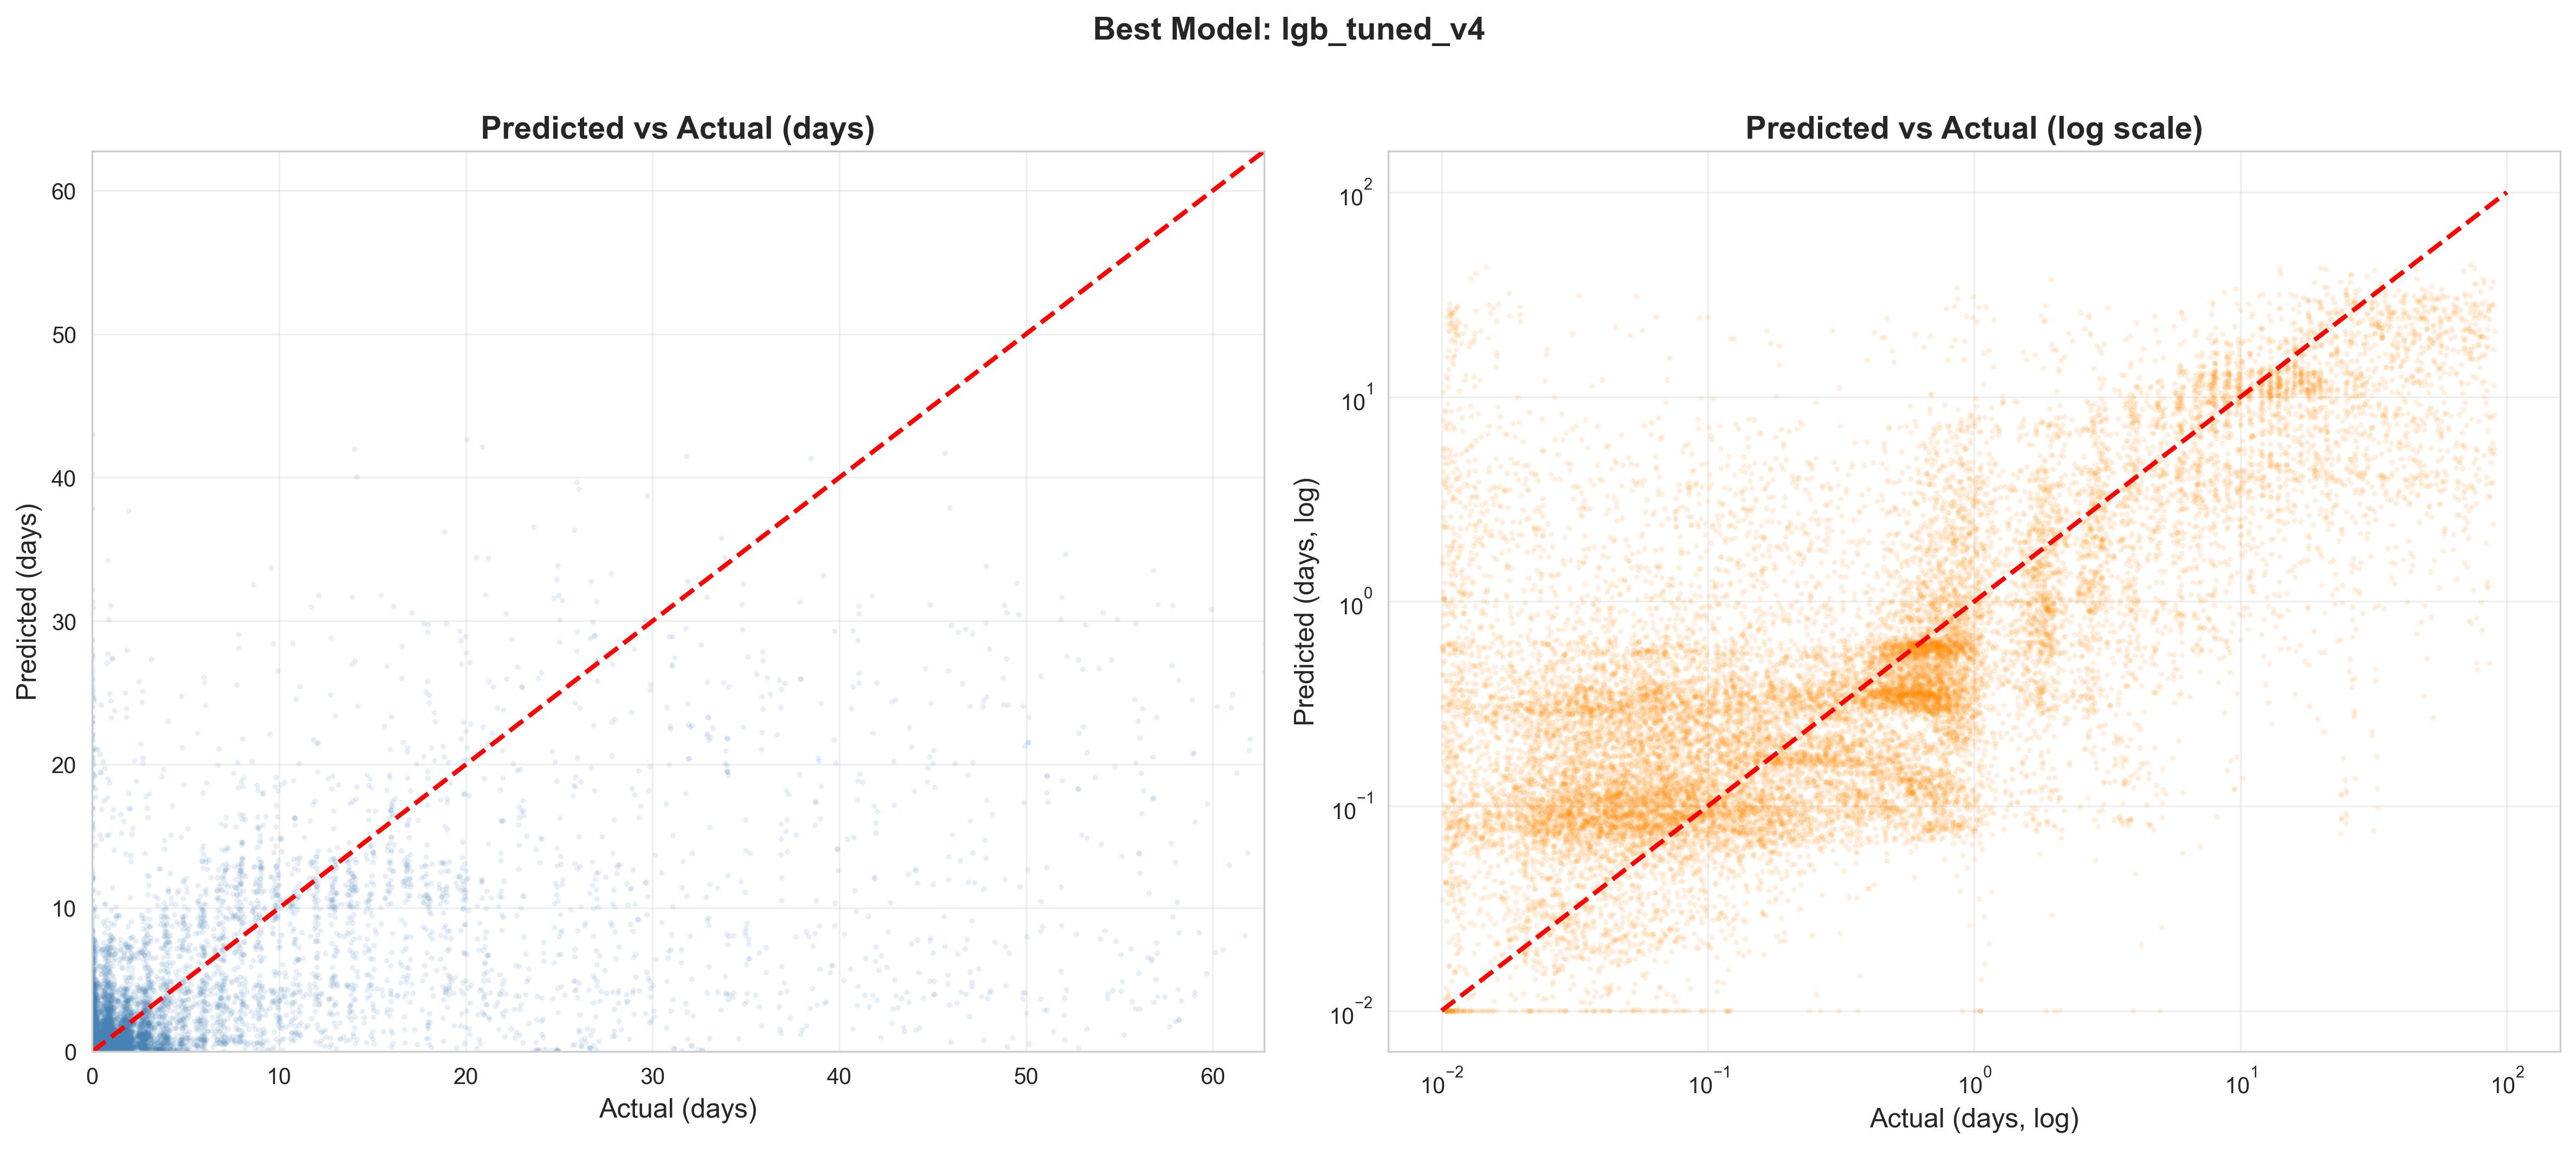
\includegraphics[width=\columnwidth]{figures/predicted_vs_actual_v4.png}
\caption{Predicted vs.\ actual resolution time (tuned LightGBM,
test set). The diagonal indicates perfect prediction. The model
concentrates predictions in the short-duration region, consistent
with the target distribution.}
\label{fig:predvsactual}
\end{figure}

%% ================================================================
\section{Discussion}
\label{sec:discussion}
%% ================================================================

\subsection{Comparison with Prior Work}

The individual-request prediction approach taken here
differs fundamentally from SWIFT's aggregate forecasting
paradigm~\cite{raj2021swift}. Where SWIFT produces a single
weekly resolution time estimate applicable to all requests in a
given period, the present approach generates distinct predictions
for each request based on its specific type, location,
department, and the operational state of the city at the time of
submission.

This distinction has practical implications: a per-request model
can inform triage decisions (e.g., flagging requests likely to
exceed SLA thresholds), whereas a weekly aggregate forecast can
only inform period-level resource planning. The 24.8\%
improvement over SARIMA provides evidence that per-request
features carry substantial predictive information beyond what
temporal patterns alone capture, but direct comparison with
SWIFT's reported GCRF performance is not attempted due to
differences in city, time period, and evaluation granularity.

The finding that tree-based methods dominate is consistent with
the broader literature on tabular prediction~\cite{
grinsztajn2022trees, shwartzziv2022tabular}. The marginal
advantage of CatBoost over LightGBM (0.03\,d MAE difference)
may reflect CatBoost's ordered boosting mechanism providing
slightly better regularization on this categorically-rich dataset,
though the difference is small enough to be sensitive to
random variation.

\subsection{Performance Plateau Analysis}

The most striking result is the performance plateau beyond
single-model tuning. Multiple sophisticated
approaches---ensemble blending, hurdle models, deeper Optuna
tuning (50 trials vs.\ 30), and recency-weighted
training---fail to improve upon the tuned single-model baseline
(MAE $\approx$~2.70\,d). Only CatBoost with MAE loss achieves a
modest additional gain of 0.03\,d.

This plateau is consistent with irreducible operational variance.
Resolution time depends on factors absent from the available
data: staffing levels and shift schedules, weather conditions
affecting outdoor work, equipment availability and maintenance
schedules, the actual severity of each reported issue (not
captured in the standardized TYPE field), and inter-request
dependencies when multiple issues compete for the same crew.
These unobserved factors impose a floor on achievable prediction
error that additional model complexity cannot overcome.

The plateau provides useful guidance for deployment: a well-tuned
single gradient boosting model with appropriate loss function
captures nearly all available predictive signal. Investment in
complex ensemble architectures yields negligible returns compared
to investment in richer data sources.

\subsection{Spatial Feature Contribution}

The SHAP analysis reveals that raw geographic features
(latitude, longitude, distance from city center) contribute
modestly to prediction accuracy compared to organizational
features (department, request type, historical resolution
patterns). This does not mean that space is irrelevant---rather,
the spatial signal is effectively captured by categorical
variables that correlate with location. A request's type and
responsible department are partially determined by its location,
and historical resolution statistics by type and department
implicitly encode spatial service patterns.

This finding suggests that for 311~resolution time prediction,
the primary spatial structure operates through the institutional
geography of municipal service delivery (department boundaries,
crew assignments, facility locations) rather than through
continuous spatial fields. Future work incorporating explicit
spatial process models or point-pattern analysis might extract
additional spatial signal, but the current results indicate that
categorical proxies capture the dominant spatial effects.

\subsection{Deployment Implications}

A production deployment of per-request resolution time
prediction would require several considerations:

\textbf{Real-time feature computation.} Operational features
(backlog, velocity, workload) must be updated in near-real-time
from the live 311~database. The one-day lag built into the
feature engineering pipeline provides a natural buffer, but
infrastructure for daily batch computation or streaming updates is
needed.

\textbf{Model retraining cadence.} Walk-forward results suggest
stable performance over 2--3 year horizons, but major operational
changes (new departments, policy shifts, technology upgrades)
would necessitate retraining. A quarterly or semi-annual retrain
schedule appears sufficient for stable environments.

\textbf{Prediction uncertainty.} The current model produces point
estimates. For operational use, prediction intervals
(available via the quantile regression variant) would provide
more actionable information, allowing agencies to communicate
ranges rather than precise estimates to residents.

\textbf{Equity monitoring.} Given documented socio-spatial
disparities in 311~reporting behavior~\cite{kontokosta2021bias},
deployed predictions should be monitored for systematic bias
across neighborhoods and demographic groups. A model trained on
biased service delivery patterns may perpetuate or amplify
existing inequities if used to allocate resources.

%% ================================================================
\section{Limitations}
\label{sec:limitations}
%% ================================================================

\textbf{Single-city scope.} All results are specific to Boston's
operational patterns, departmental structure, and service request
taxonomy. Transfer to other municipalities would require
retraining and potentially redesigning category-specific features.

\textbf{Log retransformation bias.} Training on $\log(1+x)$ and
back-transforming via $\exp(\hat{y})-1$ introduces systematic
underestimation for large values due to Jensen's
inequality. Alternative approaches such as direct MAE
optimization or smearing estimators~could mitigate this bias.

\textbf{ARIMA comparison asymmetry.} The 24.8\% improvement over
SARIMA reflects a genuine methodological advantage (per-request
features vs.\ aggregate forecasts) rather than a like-for-like
model comparison. The improvement figure should not be
interpreted as indicating that gradient boosting is 24.8\% better
than GCRFs for the same prediction task.

\textbf{Walk-forward consistency.} Walk-forward models do not use
early stopping (unlike the main pipeline), introducing a minor
methodological inconsistency. The MAE range (2.43--2.66\,d)
should be interpreted as a stability check rather than a precise
performance estimate.

\textbf{Missing operational covariates.} The most impactful
limitation is the absence of staffing, weather, equipment, and
severity data. These factors likely account for much of the
irreducible variance that constrains prediction accuracy.

\textbf{Geographic distance approximation.} The Euclidean
distance feature on raw coordinates slightly distorts distances
at Boston's latitude ($\sim$26\% longitude compression). This
has negligible impact on tree-based splits but would affect
distance-based models or kernel methods.

\textbf{Reporting bias.} As documented by Kontokosta and
Hong~\cite{kontokosta2021bias}, 311~data reflects reporting
behavior rather than ground-truth service need. The model is
trained on and predicts resolution times for \emph{reported}
requests, not the underlying universe of service issues.

%% ================================================================
\section{Conclusion and Future Work}
\label{sec:conclusion}
%% ================================================================

This study demonstrates that per-request gradient boosting models
can predict 311~service request resolution time with an MAE of
2.67~days (33.3\% improvement over the mean baseline) using 99
features available at request creation time. The approach
substantially outperforms ARIMA/SARIMA time-series models and
exhibits stable performance across three annual walk-forward
folds.

The performance plateau observed beyond single-model tuning
provides strong evidence that the current feature set captures
nearly all available predictive signal, and that further gains
require richer data sources rather than more complex models. SHAP
analysis reveals that the spatial signal in resolution time
operates primarily through organizational and categorical
structure rather than raw coordinates---a finding relevant to the
broader urban computing community studying how cities deliver
services across space.

Several directions for future work emerge:

\textbf{External data integration.} Incorporating weather data,
city staffing schedules, and road/infrastructure condition
datasets could address the irreducible variance identified in
this study, potentially breaking through the performance plateau.

\textbf{Spatial process models.} Explicit modeling of spatial
autocorrelation in resolution times---e.g., through geographically
weighted regression or spatial random effects---could extract
spatial signal not captured by categorical proxies. The current
finding that raw geographic features contribute modestly does not
rule out the presence of more complex spatial structure
accessible through purpose-built spatial models.

\textbf{Multi-city transfer learning.} Extending the approach to
multiple cities could test the generalizability of the feature
engineering pipeline and identify which features transfer across
municipal contexts. City-specific features (department names,
request taxonomies) would require adaptation, but temporal and
operational patterns may generalize.

\textbf{Survival analysis.} Modeling resolution time as a
survival process rather than a point prediction could more
naturally handle the right-censored structure (90-day cap) and
provide time-to-event probabilities useful for SLA monitoring.

\textbf{Fairness-aware prediction.} Given documented reporting
biases~\cite{kontokosta2021bias}, developing fairness-constrained
prediction models that account for socio-spatial disparities
represents an important direction for equitable deployment.

%% ================================================================
\balance
\bibliographystyle{ACM-Reference-Format}
\bibliography{references}

\end{document}
